\documentclass{article}
\usepackage{xspace,graphicx,amsmath,amsthm,amssymb,xcolor}
\usepackage{listings}
\usepackage{wrapfig}
\usepackage{hyperref}

\setlength{\topmargin}{0.1in}
\setlength{\oddsidemargin}{0in}
\setlength{\evensidemargin}{0in}
\setlength{\headheight}{0in}
\setlength{\headsep}{0in}
\setlength{\textheight}{9in}
\setlength{\textwidth}{6.5in}
\newenvironment{Question}[2][Question]{\begin{trivlist}
\item[\hskip \labelsep {\bfseries #1}\hskip \labelsep {\bfseries #2.}]}{\end{trivlist}}
\title{CS531 Programming assignment \#1}
\author{Matt Meyn, Durga Harish, and Jon Dodge}


\begin{document}
\maketitle
\section{Abstract}

In this paper, we have implemented three types(simple reflex, Random, Deterministic agents ) of vacuum cleaning agents in two  different environmental setting(Fig. 1).   The first variant (Env-1) of environment has no interior rooms and the other variants (Env-2A,2B,4) have 4 interior rooms. Env-4 has walls which are offset from each other.   Simple reflex agent has no memory element in it, whereas  deterministic agent has 3 bits of memory to store information about current state and history.  The performance of the vacuum cleaning agent is calculated based on two statistics (Percentage clean: $\frac{No.\thinspace  of\thinspace  cleaned \thinspace cells}{Total\thinspace  no.\thinspace  of\thinspace  dirty \thinspace cells}$, Efficiency:$\frac{No.\thinspace  of \thinspace cleaned \thinspace cells}{Total\thinspace actions}$).   We saw simple reflex agent has higher efficiency compared to the deterministic agent in Envi-1.  On other hand, the deterministic agent is able to clean more cells compared to the simple reflex agent.  We also observed that the simple reflex agent got stuck( not coming back home ) in Eniv-2B.  We tuned parameters of a random agent and calculated the performance in each setting. Finally, we presented our ideas on building a more efficient vacuum cleaning agent in complex environment.  



\section{Introduction}
The goal of this project is to assess the results of various agent control strategies in a simple path planning domain in different environments.Specifically, we created a simulation of a self-moving vacuum cleaner that must clean as many spaces as possible in a discrete environment of 10 by 10 spaces.
The three strategies we explore are
\begin{enumerate}
\item Memoryless deterministic reflex agent
\item Randomized reflex agent
\item Deterministic Model-based reflex agent\\

In this experiment we are considering two types of environments of 10X10 grid(Fig 1).  One environment has no interior walls(Env-1), whereas other one is divided in four rooms(Env-2A,Env-2B).  We have three percepts (Wall Sensor, dirt sensor, home sensor).  Initially every cell has dirt to be cleaned. \\

The performance of the agent is evaluated on two statistics (Percentage clean: $\frac{No.\thinspace  of\thinspace  cleaned \thinspace cells}{Total\thinspace  no.\thinspace  of\thinspace  dirty \thinspace cells}$, Efficiency:$\frac{No.\thinspace  of \thinspace cleaned \thinspace cells}{Total\thinspace actions}$).  The Agent is shut-off once it reaches home cell. 
\end{enumerate}



\section{Description of agents}
We tested three different agents. Each of them has the same set of environments to clean, the same set of possible percepts as described above, and the same set of actions it can take. In general, available actions are to move, turn left, and turn right, though the existence of a wall may remove the availability of the move option. The differences among the three agents are of course the availability of 3 bits of memory in the model-based reflex agent, and the rules by which each agent chooses its next action. The rules for each agent are as follows:

\subsection{Memoryless deterministic reflex agent}
Essentially, this agent will move forward until it faces a wall, then turn right.

\begin{lstlisting}[frame=single]		
	if not isFacingWall:
		return Move
			
	if isHome:
		return TurnOff
	else:
		return TurnRight
\end{lstlisting}

\begin{figure}[h!]
\centering
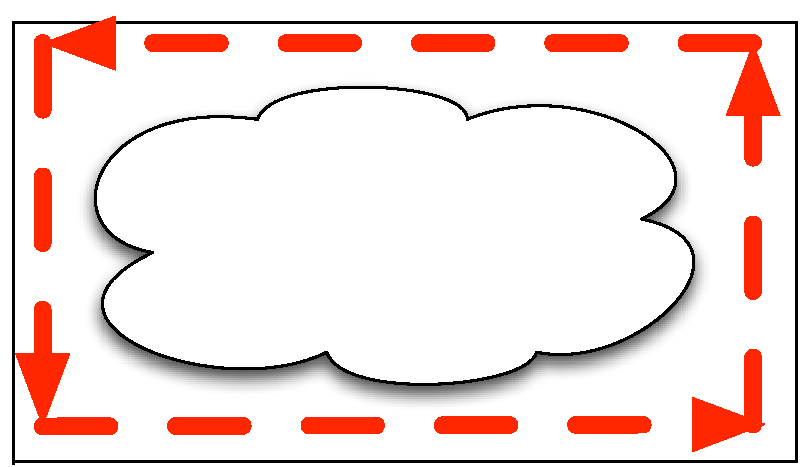
\includegraphics[width=.5\linewidth]{reflex.pdf}
\caption{Illustrates the search path of the memoryless deterministic reflex agent.  Note that the part inside the outermost ring of the environment will not be cleaned.}
\label{fig:reflex}
\end{figure}


\subsection{Randomized reflex agent}
If this agent encounters a dirty space in the grid, it cleans it. If it finds itself facing a wall, it turns in a random direction (equal probability right and left). Otherwise, the agent proceeds by weighted coin tosses.




\begin{lstlisting}[frame=single]
if isHome:
	if random.randint(0, 100) < self.probTurnOff:
		return self.ActTurnOff

if isFacingWall:
	randNum = random.randint(0, self.probTurnLeft + self.probTurnRight)
	if randNum < self.probTurnLeft:
		return self.ActTurnLeft
	else:
		return self.ActTurnRight

else:
	randNum = random.randint(0,100)
	if randNum < self.probTurnLeft:
		return self.ActTurnLeft
	elif randNum < self.probTurnLeft + self.probTurnRight:
		return self.ActTurnRight
	else:
		return self.ActMove
\end{lstlisting}



\subsection{Deterministic Model-based reflex agent}
In this case we implemented a snaking space-filling curve.  The agent will traverse vertically "north" till it hits the wall, after which it takes a right turn, moves forward one space, turns right again and continues moving forward in the "south" direction. When moving in this direction, the turns become left turns.  Eventually, this path will be exhausted, and we flip the reverse bit so that we go back down the same path we came in on.

We are using  four Boolean variables (IsSweepingNorth, isStartingTurn, isDoneTurning, isReversed) to keep track of action dynamics of the agent. Note that the first boolean variable could be removed if we added a compass sensor to the robot.  Additionally, we have an implementation using 3 booleans (slightly different implementation) commented out in our submission.  It stores the previous move as well as the desired next move in order to handle the dynamics of making the U turn, which takes some state information to perform.

The description of the variables are below: 
\begin{enumerate}
\item IsSweepingNorth = True if agent moving in North, is False if moving in South. Determines whether the agent turns left or right when it hits the wall.
\item isStartingTurn - Indicates whether we have begun a U turn
\item isDoneTurning - Indicates whether the U turn has been completed.
\item isReversed - Lets us know when our space filling curve has hit the wall and needs to come back along the same path 
\end{enumerate}

\begin{figure}[h!]
\centering
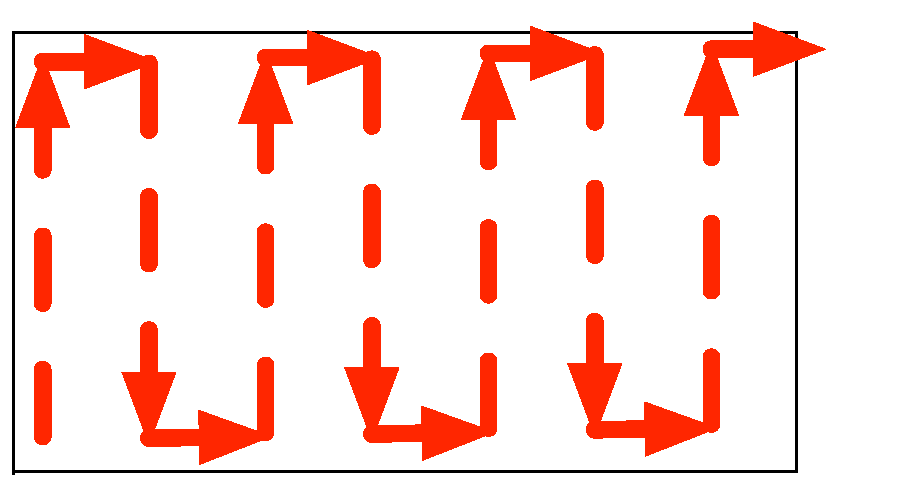
\includegraphics[width=1\linewidth]{snaking}
\caption{Illustrates the search path of the model-based reflex agent.  Refer to the source code for additional information about what each rule handles.  Rules 2-4 handle the first U turn, while 5,3,6 handle the next.  7-10 handle some edge cases where we must bounce off the opposing wall and return along the same path we came on.}
\label{fig:reflex}
\end{figure}
\clearpage

\begin{lstlisting}[frame=single]
if self.SenseHome() and self.isReversed:
	return self.ActTurnOff

if not hitWall and not turnStarted and turnDone:  # Rule 1
	return self.ActMove

if hitWall and not turnStarted and turnDone and sweepingNorth: # Rule 2
	self.isStartingTurn = True; self.isDoneTurning = False
	return self.ReversedTurn(Directions.RIGHT)

if not hitWall and turnStarted and not turnDone:	 # Rule 3
	self.isStartingTurn = False
	return self.ActMove

if not hitWall and not turnStarted and not turnDone and sweepingNorth: # Rule 4
	self.isDoneTurning = True; self.isSweepingNorth = False
	return self.ReversedTurn(Directions.RIGHT)

if hitWall and not turnStarted and turnDone and not sweepingNorth: # Rule 5
	self.isStartingTurn = True; self.isDoneTurning = False
	return self.ReversedTurn(Directions.LEFT)

if not hitWall and not turnStarted and not turnDone and not sweepingNorth: # Rule 6
	self.isDoneTurning = True;self.isSweepingNorth = True
	return self.ReversedTurn(Directions.LEFT)

if hitWall and not turnStarted and not turnDone and sweepingNorth: # Rule 7
	self.isDoneTurning = True; self.isSweepingNorth = False
	return self.ReversedTurn(Directions.RIGHT) 

if hitWall and turnStarted and not turnDone and sweepingNorth: # Rule 8
	self.isReversed = True; self.isDoneTurning = True
	self.isStartingTurn = False; self.isSweepingNorth = False
	return self.ReversedTurn(Directions.LEFT) 

if hitWall and not turnStarted and not turnDone and not sweepingNorth: # Rule 9
	self.isDoneTurning = True; self.isSweepingNorth = True
	return self.ReversedTurn(Directions.LEFT) 

if hitWall and turnStarted and not turnDone and not sweepingNorth: # Rule 10
	self.isReversed = True; self.isDoneTurning = True
	self.isStartingTurn = False; self.isSweepingNorth = True
	return self.ReversedTurn(Directions.RIGHT) 
\end{lstlisting}



\section{Experimental Setup}
We have conducted experiments in two different types of environments.
The first is a square room full of dirt with no interior walls, while the remainder are divided by walls into four sub-rooms, to make navigation more difficult. Each pair of adjacent rooms is connected by a gap or "doorway" in the wall.

\begin{figure}[h!]
\centering
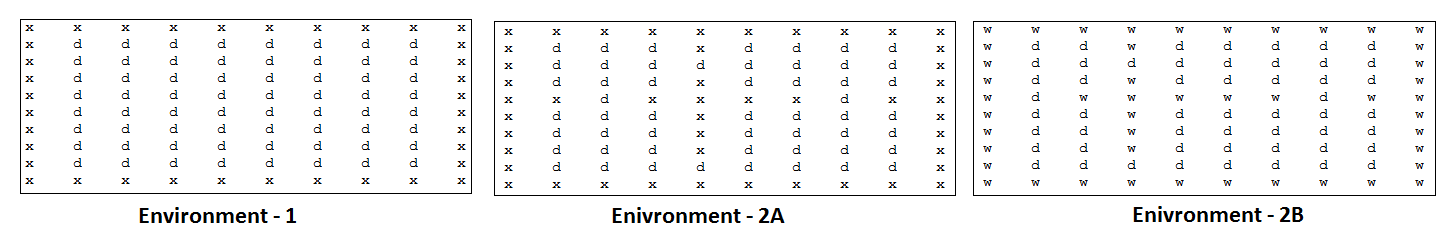
\includegraphics[width=1\linewidth]{different_evirnoments.png}
\caption{Shows different environments, where x denotes a wall and d denotes a dirt cell.}
\label{fig:environments}
\end{figure}

Agents 1 and 3 are deterministic, so they will be run once for each environment, while the second agent is uses randomness, so we will report the results of 50 trials.  We chose two sets of parameters for our random agent, one where move, turn left, and turn right are all given equal probabilities (Random Agent 1), and another set where move is given 70\% weight, and turns are given 15\% each (Random Agent 2 - Move).

The agent is terminated( turned off) when it reaches home cell, or if it spends 10,000 actions.



\section{Results}
We carried out the experiment with 3 agents (Simple Reflex Agent, Random Agent, Deterministic Agent with 3 bits of memory) and 3 different Environments, Figure~\ref{fig:environments} shows the different types of the environments used to experiment.    In order to calculate the performance of random agent, we ran for 50 trials and took an average. Tables 1-4 show the agents performance in each environment.  

\begin{figure}[h!]
\centering
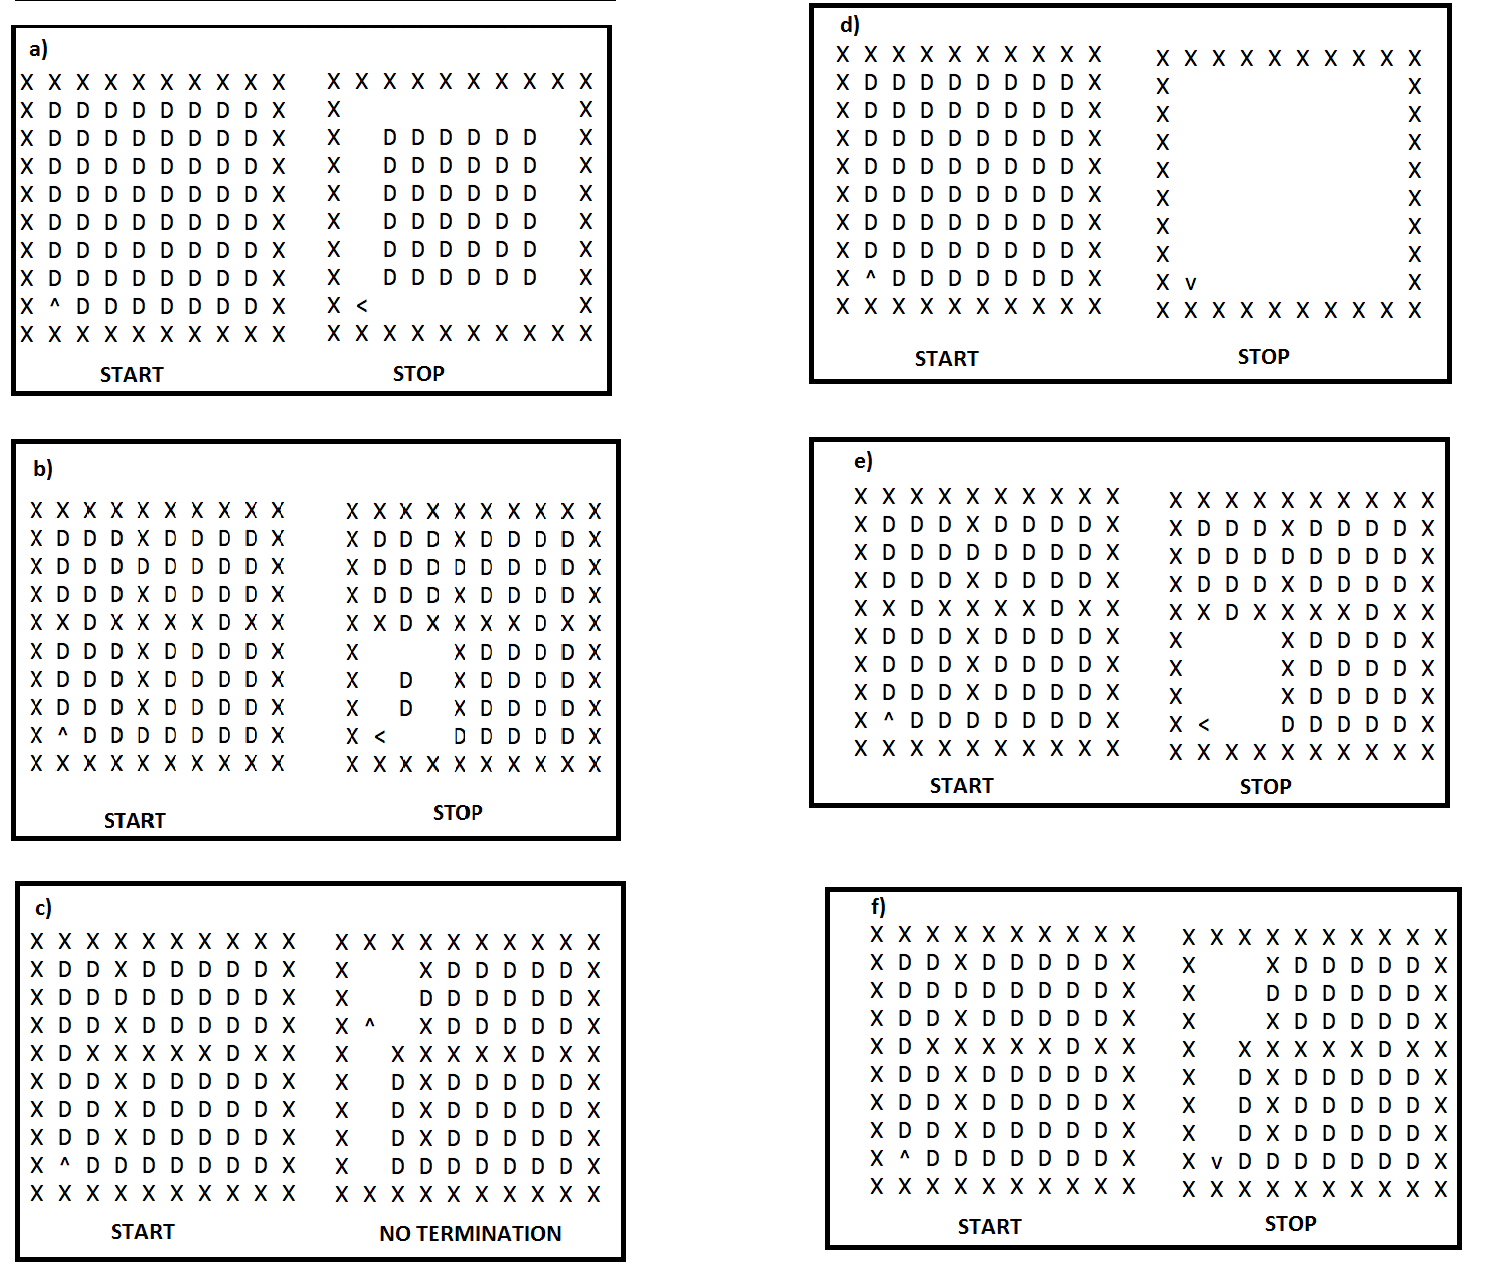
\includegraphics[width=1\linewidth]{all_in_one}
\caption{Shows different environments after cleaning, where x denotes a wall and d denotes a dirt cell.}
\label{fig:cleaned}
\end{figure}



\begin{table}[h!]
\centering
\caption{Different Agents Performance in Environment-1. There are 64 dirty cells in this environment}
\label{my-label}
\begin{tabular}{l|ll|ll}
\hline
                    & \# Cleaned Cells & \# Actions  & \% Clean & Cleaned/Actions \\ \hline
Simple Reflex Agent 		& 28                  & 60                  & 43.75     & 0.46            \\ \hline
Random Agent 1       	& 17          	& 221                & 27.8       & .08            \\ 
Random Agent 2 - Move 	& 23 			& 133		&37.25	& .18			\\ \hline
Model Agent 		& 64                  & 221                & 100       & 0.29            \\ \hline
\end{tabular}
\end{table}




\begin{table}[h!]
\centering
\caption{Different Agents Performance in Environment-2A. There are 53 dirty cells in this environment}
\label{my-label}
\begin{tabular}{l|ll|ll}
\hline
                    & \# Cleaned Cells & \# Actions  & \% Clean & Cleaned/Actions \\ \hline
Simple Reflex Agent 		& 10                  & 24                  & 18.9     & 0.42            \\ \hline
Random Agent 1       	& 6	         	& 172                & 12.9       & .039            \\ 
Random Agent 2 - Move 	& 10 			& 71		& 19.8	& .15			\\ \hline
Model Agent 		& 22                  & 10000                & 41.5       & .0022            \\ \hline
\end{tabular}
\end{table}

\begin{table}[h!]
\centering
\caption{Different Agents Performance in Environment-2B. There are 53 dirty cells in this environment}
\label{my-label}
\begin{tabular}{l|ll|ll}
\hline
                    & \# Cleaned Cells & \# Actions  & \% Clean & Cleaned/Actions \\ \hline
Simple Reflex Agent 		& 13                  & 10000                  & 24.5     & .0013            \\ \hline
Random Agent 1       	& 9	         	& 150                & 17.9       & .06            \\ 
Random Agent 2 - Move 	& 15 			& 119		& 29 	& .13			\\ \hline
Model Agent 		& 14                  & 51                & 26.4       & .27            \\ \hline
\end{tabular}
\end{table}

\begin{table}[h!]
\centering
\caption{Different Agents Performance in Environment-4. There are 55 dirty cells in this environment}
\label{my-label}
\begin{tabular}{l|ll|ll}
\hline
                    & \# Cleaned Cells & \# Actions  & \% Clean & Cleaned/Actions \\ \hline
Simple Reflex Agent 		& 6                  & 16                  & 10.9     & .375            \\ \hline
Random Agent 1       	& 8	         	& 177                & 14.8       & .046            \\ 
Random Agent 2 - Move 	& 11 			& 84		& 20.2 	& .13			\\ \hline
Model Agent 		& 35                  & 10000                & 63.6       & .0035            \\ \hline
\end{tabular}
\end{table}

\section{Discussion}


%%%%%%%%%%%%%%%%%%%%%%%%%%%%%%%%%%%%%%%%%%%%%%%%%%%%%%%%%%%%%%%%%%%%%%%%%%%%%%%%%%%%%%%%%%%%%%%%%%%%%%%%%%
\begin{Question}{3}What is the best possible performance achievable by the simple reflex agent in the two environments? What prevents it from achieving the goal of cleaning the room perfectly in each case?\\

\begin{enumerate}
\item The simple reflex agent performed best in Environment-1 (Cleaned Cells: 28, No. of actions: 60) compared to other  Environments.  We observed that simple reflex agent failed in Environment 2B as the agent got trapped in a particular room.  Figure 4 depicts the Start and the place where the agent got trapped.  
\item The reflex agent has very limited performance in any environment because it can act only on the information available to its sensors  at the current time. Therefore, it has limited navigation abilities. There really is no other reasonable action for it to take other than move forward if its path is not blocked; turn if its path is blocked; and shut off if it is home.
\end{enumerate}

\end{Question}


%%%%%%%%%%%%%%%%%%%%%%%%%%%%%%%%%%%%%%%%%%%%%%%%%%%%%%%%%%%%%%%%%%%%%%%%%%%%%%%%%%%%%%%%%%%%%%%%%%%%%%%%%%
%%%%%%%%%%%%%%%%%%%%%%%%%%%%%%%%%%%%%%%%%%%%%%%%%%%%%%%%%%%%%%%%%%%%%%%%%%%%%%%%%%%%%%%%%%%%%%%%%%%%%%%%%%
\begin{Question}{4}How well does the random agent perform? Tune any parameters of the random agent to improve its performance. Give a table showing the number of actions it took to clean 90 of the room for each trial. What is the average of these numbers for the best 45 trials? What are the costs and benefits of randomness in agent design?\\
\begin{enumerate}
\item 

In Environment 1, the randomized agent performs worst by any measure. It cleans fewer spaces and does so using more actions. In a more complex environment (one with interior walls), the randomized agent cleans a larger number of spaces than the other agents, although it uses many more actions to do so. 

We tested the randomized agent with three different sets of parameters. In the first test, the agent, when not facing a wall, had a 1 in 3 chance of turning rather than moving forward; in the second, a 1 in 10 chance; in the third test, a 2 in 3 chance of turning rather than moving forward. Of the three, the agent performed most effectively with a 1 in 3 chance of moving forward. The worst performance was observed when the probabilities were reversed and the agent had a 2 in 3 chance of turning. Unsurprisingly, this resulted in many wasted actions as the machine turned far more often than necessary.  It is fairly clear that when the robot favors movement over turning, it achieves a better result.

The link \url{http://bit.ly/2k67CAh}  has the tables showing the number of actions it took to clean 90\% of the room for each trial.

The advantage of a randomized agent appears to be that it can generate seemingly more complex behavior than the reflex agents, which easily fall into simple repeating patterns of movement which can make them unable to access large parts of a complex environment. Thus, the random agent can (eventually) reach most or all of the spaces in a room, but at a cost. When the model-based agent was not the best, the random one was.
\end{enumerate}


\begin{table}[h!]
\centering
\caption{Illustrate the performance of Random Agent in Environment-1}
\label{my-label}
\begin{tabular}{|l|l|l|l|}
\hline
                                                                                        & 90 \% clean & Avg. \# of Actions & $\frac{clean}{Actions}$ \\ \hline
\begin{tabular}[c]{@{}l@{}}$p=\frac{1}{3}$, Turning\\ $p=\frac{2}{3}$,Move\end{tabular} & 58          & 358.77             & 0.16                    \\ \hline
\begin{tabular}[c]{@{}l@{}}$p=\frac{1}{3}$, Turning\\ $p=\frac{2}{3}$,Move\end{tabular} & 58          & 513.818            & 0.11                    \\ \hline
\begin{tabular}[c]{@{}l@{}}$p=\frac{1}{3}$, Turning\\ $p=\frac{2}{3}$,Move\end{tabular} & 58          & 1219.26            & 0.04                    \\ \hline
\end{tabular}
\end{table}




\begin{table}[h!]
\centering
\caption{Illustrate the performance of Random Agent in Environment-2A}
\label{my-label}
\begin{tabular}{|l|l|l|l|}
\hline
                                                                                        & 90 \% clean & Avg. \# of Actions & $\frac{clean}{Actions}$ \\ \hline
\begin{tabular}[c]{@{}l@{}}$p=\frac{1}{3}$, Turning\\ $p=\frac{2}{3}$,Move\end{tabular} & 47          & 642.92             & 0.07                    \\ \hline
\begin{tabular}[c]{@{}l@{}}$p=\frac{1}{3}$, Turning\\ $p=\frac{2}{3}$,Move\end{tabular} & 47          & 835.24             & 0.05                    \\ \hline
\begin{tabular}[c]{@{}l@{}}$p=\frac{1}{3}$, Turning\\ $p=\frac{2}{3}$,Move\end{tabular} & 47          & 1973.82            & 0.02                    \\ \hline
\end{tabular}
\end{table}

\begin{table}[h!]
\centering
\caption{Illustrate the performance of Random Agent in Environment-2B}
\label{my-label}
\begin{tabular}{|l|l|l|l|}
\hline
                                                                                        & 90 \% clean & Avg. \# of Actions & $\frac{clean}{Actions}$ \\ \hline
\begin{tabular}[c]{@{}l@{}}$p=\frac{1}{3}$, Turning\\ $p=\frac{2}{3}$,Move\end{tabular} & 47          & 555.35             & 0.08                    \\ \hline
\begin{tabular}[c]{@{}l@{}}$p=\frac{1}{3}$, Turning\\ $p=\frac{2}{3}$,Move\end{tabular} & 47          & 572.6              & 0.08                    \\ \hline
\begin{tabular}[c]{@{}l@{}}$p=\frac{1}{3}$, Turning\\ $p=\frac{2}{3}$,Move\end{tabular} & 47          & 2322.64            & 0.02                    \\ \hline
\end{tabular}
\end{table}


\end{Question}



%%%%%%%%%%%%%%%%%%%%%%%%%%%%%%%%%%%%%%%%%%%%%%%%%%%%%%%%%%%%%%%%%%%%%%%%%%%%%%%%%%%%%%%%%%%%%%%%%%%%%%%%%%

%%%%%%%%%%%%%%%%%%%%%%%%%%%%%%%%%%%%%%%%%%%%%%%%%%%%%%%%%%%%%%%%%%%%%%%%%%%%%%%%%%%%%%%%%%%%%%%%%%%%%%%%%%
\begin{Question}{5}How does the model-based deterministic agent perform in the two environments? Is it able to clean the room perfectly? How long does it take? Can the agent be improved with more memory?\\

\begin{enumerate}
\item The memory-based deterministic agent is able to completely clean Environment 1 (with no interior walls), but cannot completely clean Environments 2A and 2B. In Environment 1, it does clean 100 percent of the room, but it takes 221 actions to do so, leading to an efficiency score of 0.28 as opposed to the simple reflex agent's score of 0.46.

In most of our tests, the model-based agent resulted in the cleanest room, but occasionally its efficiency suffered.

We strongly suspect that the memory-based agent could have better performance given more memory. The 3 bits of memory our agent has are sufficient to remember instructions on what movement to take next (move forward, turn) and to detect corners. But with more memory it would be possible to detect doorways, remember where they are, remember where the home cell is, and also remember how many spaces have been cleaned. Essentially, given substantial memory resources, we can build a map as we traverse the environment.  To conclude, knowing and remembering the current state of the environment would enable an agent to clean more dirty spaces and to navigate more efficiently.
\end{enumerate}

\end{Question}


%%%%%%%%%%%%%%%%%%%%%%%%%%%%%%%%%%%%%%%%%%%%%%%%%%%%%%%%%%%%%%%%%%%%%%%%%%%%%%%%%%%%%%%%%%%%%%%%%%%%%%%%%%



 \begin{Question}{6}What are the tradeoffs between the random and deterministic agents? How would you design better agents for more complex environments, say with polygonal obstacles?\\
 \begin{enumerate}
 \item Although our deterministic agents generally performed more efficiently than the randomized one, they suffered from a major shortcoming: in an environment with interior walls, they can become stuck in repeating patterns. With the lack of memory in our deterministic agents, there is noway to detect these kind of patterns.  In contrast, the ranodmized agent does not require memory to get out of looping patterns, because it basically has no predetermined patterns of movement. The behavior of the random agent thus can be expected to terminate eventually in any situation where there exists a path to the home cell.
 
 We believe having more information about environment, it is possible to solve for more complex situations.storing the blueprint of the environment in a matrix form; current co-ordinates of the agent, and predicting the future path with the current state information.    
 \end{enumerate}
 \end{Question}

\begin{Question}{7}What did you learn from this experiment? Were you surprised by anything? \\

\begin{enumerate}
 \item We were surprised to discover how little complexity of behavior could be generated from three percepts and three bits of memory. In the end, we found the two deterministic reflex agents (with and without memory) to be somewhat unsatisfactory because they could not be guaranteed to terminate the program in every environment. We discovered that lack of memory not only makes it difficult to know much about the enviromnent, but also makes it difficult to implement behavior of any real complexity because there is no way to store sequences of actions longer than one or two ahead. 
 
We found it surprisingly difficult to get the robot back to the home square with so little state information.  Without being able to even store a square index, having any kind of accurate location information was a real challenge.

\end{enumerate}
\end{Question}



\begin{figure}[h!]
\centering
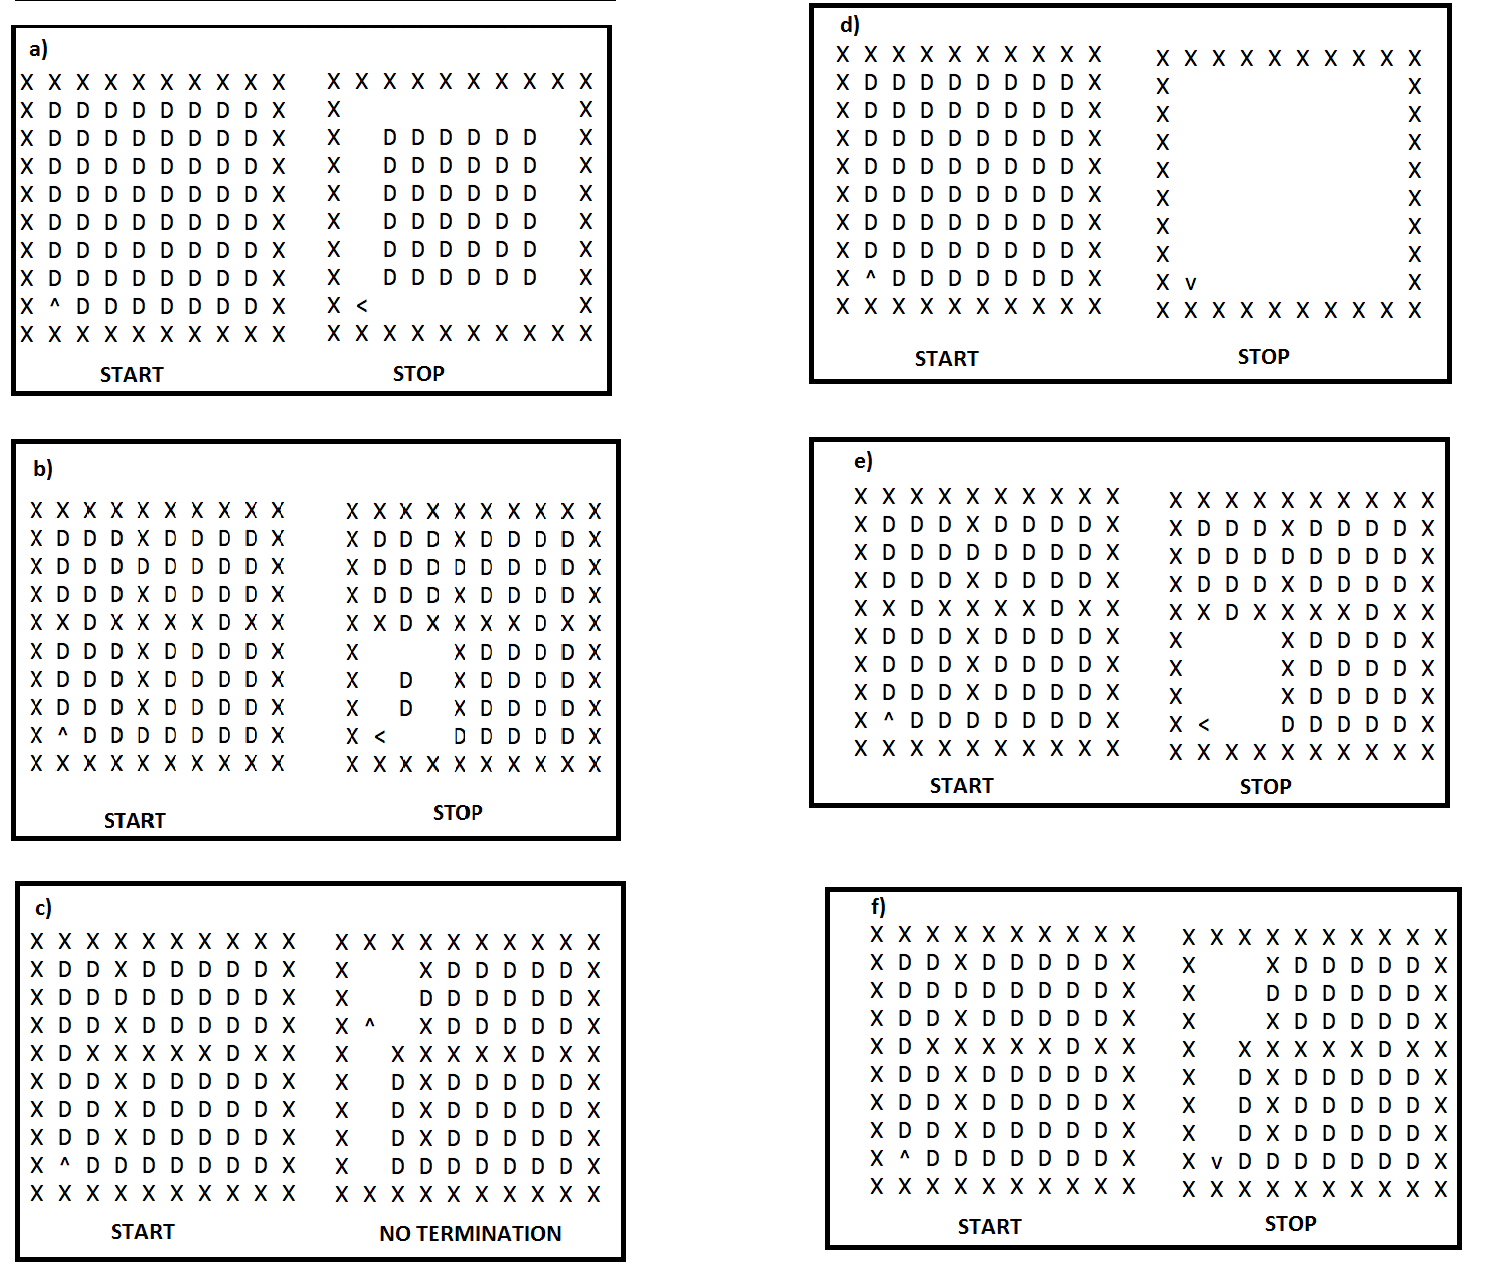
\includegraphics[width=1\linewidth]{all_in_one.png}
\caption{Part a),b) c) of figure shows the start and stop position of simple reflex vacuum cleaner agent in Env-1, Env-2A, Env-2B respectively. Part d), e), f) depicts the start and stop position of 3-bit deterministic agent in Env-1, Env-2A, Env-2B Respectively.}
\label{fig:method}
\end{figure}


\end{document}